\documentclass{article}
\usepackage{darkmode}
\usepackage{amsmath}
\usepackage{amssymb}
\usepackage{hyperref}
\usepackage{gensymb}
\usepackage{tikz}
\usetikzlibrary{calc,decorations.pathreplacing}

\enabledarkmode
\title{Astro Notes}
\author{Pierson Lipschultz}

\begin{document}

\tableofcontents

\maketitle

\section{Class overview}
Office hours tues and thurs 11-12 astro 237

ta office hours

wed 3:30:530 astro 2367

hw due wed  

hw posted week before

\begin{list}{-}{}
\item solar system 
\item steller evo
\item compact objects
\item galaxy quasi darkmatter
\item cosmic web
\item big bang
\end{list}

course goals
\begin{list}{-}{}
\item apply pys to universe
\item understand foundations of modern astro, astrophys, and cosmology
\item conceptual understanding of the uni based on physical principles
\end{list}

\section{Early Astronomy}
\subsubsection{Greek}
\begin{list}{-}{}
\item Aristotle 
    \begin{list}{-}{}
    \item earth is spherical
    \item partial lunar eclipses
    \item some stars visible from southern locations but not northern and vice versa
    \item had ideas regarding perfect geo influenced by Pythagoras and Plato
    \end{list}
\item Aristarchus (310-230 BC):
\begin{list}{-}{}
\item unpreceded heliocentric framework
\item trig distances earth-moon-sun system
\item angular diameters $\theta_{sun} \approx \theta_{moon} \therefore \frac{A}{C} = \frac{D_{moon}}{D_{moon}}$
\item diameters from lunar eclipses $D_{moon} < D_{earth}$
\end{list} 
\item Eratoshs (176-195 BC):
\begin{list}{-}{}
\item Determined radius of spherical earth $R_{E}$
\item Sun at zenith at noon on summer solstice at Aswan 
\item But further north in Alexandria, Egypt, the sun is south of the zenith by angle $\alpha$
\end{list}
\item Hipparchus (190-120 BC):
\begin{list}{-}{}
\item Discover precession of the equinoxes from examination of star catalogs over centuries
\item established the magnitude system
\end{list}
\item Copernicus (1473-1543):
\begin{list}{-}{}
\item heliocentric
\item earth rotates
\item still assumed uniform circular celestial motion 
\item inferior planets: orbit smaller than earths
\item superior planets: orbits larger than earths
\end{list}
\end{list}

\subsection{\textbf{\large Emergence of modern Astro}}

\textbf{\large Inferior planets}

\begin{list}{-}{}
\item B/C = sin $\theta_{E}$
\item B=C Sin $\theta_{E}$
\item C is AU 
\item Early astronomers didnt know C, so they could only infer rations of B/C. Ie. Orbital radii measured in AU
\end{list}

\noindent
\textbf{\large Superior Planets}

\begin{list}{-}{}
\item Measure time between opposition and eastern quadrature
\item want angle $\theta$ between opp and east quad 
\item $\theta = (\omega_{E} - \omega_{p})$ and $C/B =cos\theta$
\item measure $\tau$ and synodic period, calculate sidereal period and $\omega_{p}$; know $\omega_{E}$ and infer $C/B$
\end{list}

\noindent \textbf{\large Galilean Revolution}
\begin{list}{-}{}
\item Galileo Galilei (1564 -1642)
\item \begin{list}{-}{}
\item improved and used a basic refracting telescoping

\end{list}
\item def publication of early results 1610 \textit{"starry messenger"}
\item \begin{list}{-}{}
\item Moon is cratered; not a perfect Sphere
\item milkyway is made out of stars
\item Jupiter has moons (or as he thought, stars)
\item measured phases of Venus 
\end{list}
\end{list}

\noindent \textbf{\large Phases of Venus}
\begin{list}{-}{}
\item direct confrontation with Ptolemaic geocentric models
\item in Ptolemaic models you only see crescent phases 
\end{list}

\noindent \textbf{\large Tycho Brahe (1546-1601)}
\begin{list}{-}{}
\item Denmark, later Prague
\item Given island by king Fredrick (and staff)
\item made a accurate and vast database of celestial motion
\item had a lead nose?
\item Threw giant ragers
\item supernova named after him 
\end{list}

\noindent \textbf{\large Johannes Kepler (1571–1630, Prague)}
\begin{list}{-}{}
\item 'Inherited' (maybe stole) Brahe's data 
\item also has a SN
\item Kepler fit a new empirical model of heliocentric orbits, abandoning perfect circles 
\begin{list}{-}{}
\item ``\textit{It was as if I awoke from sleep and saw a new light}'' (Kepler, New astronomy)
\end{list}
\end{list}

\noindent \textbf{\large Kepler's Laws}

\noindent \textbf{First law}

\begin{list}{-}{}
\item The planets travel on elliptical orbits with the sun at one focus
\item Semimajor axis, half the major axis 
\item eccentricity: how elliptical (stretched) an orbit is - distance between foci divided by major axis.
\end{list}

\noindent \textbf{second law }

\begin{list}{-}{}
\item A line drawn from the sun to a planet sweeps out equal areas in equal time intervals'
\item perihelion: orbital point closet to the sun
\item aphelion: furthest orbital point from the sun
\end{list}

\noindent \textbf{third law }

Def: \textit{The square of the sidereal orbital periods of the planets are prop to the cubes of the Semimajor axis of their orbits}
\[p^2 = Ka^3\]
\begin{center}
    P = planets sidereal period\\
    a= length of semimajor axis\\
    K = constant
\end{center}

\noindent \textbf{\large Consequences of heliocentric model}
\begin{list}{-}{}
\item retrograde motion of outer planets
\item positions of outer and inner planets wrt sun
\item annual parallax 
\item aberration of starlight
\item Coriolis effect
\end{list}

\noindent \textbf{\large Parallax}
\begin{list}{-}{}
\item annual parallax: change in the apparent position when seen from two diff locations due to earth revolving around the sun. First measured by Bessel in 1838
\end{list}

\noindent \textbf{\large Aberration of starlight}
\begin{list}{-}{}
\item deflection of apparent stellar positions in the direction of the observers motion
\item analog: running throw rain and getting wet in the front and not in the back
\item detected (Picard, 1680); explained (Bradley, 1729)
\item telescope is moving along orbital vector around the sun; translation along orbit cannot exceed transit time of light through telescope
\end{list}

\noindent \textbf{\large Coriolis effect: evidence of earth rotation}
\begin{list}{-}{}
\item coriolis acceleration is perp to the direction of motion 
\item \[\vec{a_{cor}}= s\vec{v} \times \vec{\omega}\]
\item can be deduced from a pendulum
\item and in hurricanes!
\end{list}


\section{Orbital Mechanics I}
\subsection{Newtonian mechanics}
Parametric vectors\\
Displacement $\vec{r}(t) = x(t)\hat{i}y(t)\hat{j}+z(t)\hat{k}$ \\
distance: $r(t) = |\vec{r}(t)| = \sqrt{\vec{r} \cdot \vec{r}}$ \\

\subsection{Newtons laws}

First law
\begin{list}{-}{}
\item Isaac newton(1642-1727)
\item an objects' velocity remains constant unless a net outside force acts upon it
\item $\vec{v}(t) =\vec{v_0} =const$
\end{list}

second law
\begin{list}{-}{}
\item $\vec{F} = m\vec{a}(t)$
\item $\vec{F} = \frac{d\vec{p}(t)}{dt}$
\item $d\vec{v}/dt =\vec{f}/m$
\item force changes velocity
\item used a lot in computational math
\end{list}

third law
\begin{list}{-}{}
\item forces come in pairs, equal in magnitude, and opposite in direction
\end{list}

Newtonian gravity
\begin{list}{-}{}
\item a force, grav, exsits between any two objects having mass m and M, prop to the product of their masses mM and inversely proportinal tothe square of the separtation distance r of their centers
\item for coordinates centered on M:
\item $\vec{F} = -G\frac{Mm}{|\vec{r}|^2}\hat{r}$
\end{list}

\subsection{Displacement vector and polar coordinates}
\begin{list}{-}{}
\item cartesian coordinates are often written a (x,y,z) in a coordinate system centered on mass M
\item Axis orientations are chosen so that the planet orbits in the x-y plane
\item Displacement $\vec{r}(t) =x(t)\hat{i} +y(t)\hat{j}$
\end{list}

velocity vector and polar coordinates
\begin{list}{-}{}
\item unit vectors in polar coordinates vary with $\theta(t)$
\item \[\frac{d\hat{r}(t)}{dt} = \frac{d\hat{r}(t)}{d\theta} \frac{d\theta(t)}{dt} = \frac{d\theta(t)}{dt} \hat{\theta}(t)\]
\item .
\item .
\item .
\item \[\vec{v}(t) = v_r\hat{r} +v_t\hat{\theta}\]
\item two velocity components in polar coords 
\end{list}

\subsection{Kepler laws: angular momentum}
\begin{list}{-}{}
\item .
\end{list}

\subsection{keplers 2nd law = consv, angular momentum}
\begin{list}{-}{}
\item \[d\vec{L}/dt=0\]
\item \[\vec{L} =\vec{R} \times\vec{p} = \vec{r}\times m\vec{v}= const\]
\item \[\rightrightarrows |\vec{v}|=L = mrv_1\]
\end{list}

\subsection{Keplers Laws}
\subsubsection{Keplers First Law}
\begin{list}{-}{}
\item $\frac{d\vec{v}}{dt} = -\frac{GM}{r_2}\hat{r}$
\item \[\frac{L}{GMm} \frac{d\vec{v}}{dt} = \frac{d\hat{\theta}}{dt}\]
\item \[\frac{L}{GMm}\vec{v} = \hat{\theta} + e\hat{j}\]
\item take dot product of both sides with unit vector $\hat{\theta}, using$
\item $\hat{j}\cdot\hat{\theta} = \cos\theta$
\item \[\vec{v} \cdot \hat{\theta} = v_t = \frac{L}{mr}\]
\end{list}

\subsection{Kepler III}

\begin{list}{-}{}
\item we know that $\frac{dA}{dt} = \frac{l}{2m} = const$
\item area of a ellipse $a =\pi ab$ of orb period p.
\item \[\therefore \frac{A}{P} = \frac{\pi ab}{P} = \frac{L}{2m}\]
\item eclipse geo : $b^2 = a^2(1-e^2)$
\item also, $\frac{L^2}{m^2} GMa(1-e^2)$
\item \[P^2 = \frac{4\pi^2}{GM}a^3\]
\end{list}

\section{Orbital energetics}
\begin{list}{-}{}
\item total energy e is conserved 
 \begin{list}{-}{}
\item sum of K and U 
\item \[E = K+U\]
\item \[= \frac{1}{2} mv^2 - \frac{GMm}{r}\]
\end{list}
\item total E is conserved 
\item \[E = (\frac{GMm}{L})^2 \frac{m}{2}(e^2-1)\]
\item Hyperbolic orbit: $e >1, E>0, K> |U|$
\begin{list}{-}{}
\item open orbit, unbound;, single perihelion passage at $\theta = 0$
\end{list}
\item Parabolic orbit: $e = 1, E = 0, K=|U|$
\begin{list}{-}{}
\item marginally unbound; velocity approach zero at infinite time
\end{list}
\item elliptical orbit: $e<1, E<0, K = |U|$
\item objects originating outside our solar system are easily identified by their total energy 
\begin{list}{-}{}
\item measure total energy (how far away it is, how fast is it moving) 
\end{list}
\end{list}

\subsection{Checking energy in circular orbits}
\begin{list}{-}{}
\item governing equation for circular orbits in scalar from
\item \[f=ma\]
\item \[\frac{GM}{r^2} = \frac{v^2}{r} = \omega^2r\]
\item \[v = \sqrt{\frac{GM}{r}}\]
\end{list}

\subsection{Negative total energy orbits}
\begin{list}{-}{}
\item bound orbits have E < 0
\item must add energy to break ``unbind'' the orbits
\end{list}

\subsection{Parabolic orbits: escape speeds}
\begin{list}{-}{}
\item Escape speed is the speed that will bring your total pot energy to 0
\item velocity becomes zero at infinite distance
\item \[\frac{1}{2}mv^2 = \frac{GMm}{r}\]
\item \[v_{esc} = \sqrt{\frac{2GM}{r}}\]
\end{list}


\subsection{Hohmann transfer orbit}
\begin{list}{-}{}
\item Elliptical transfer orbit from earth to superior planet
 \begin{list}{-}{}
\item earths orbit becomes the transfer orbits perihelion passage
\item inserted into superior planet orbit at aphelion. This constrains launch windows
\item theoretically requires only two burns: at launch and aphelion insertion point
\end{list}
\item semimajor axis os transfer orbit 
\item \[a_{to} = \frac{a + a_{sup}}{2}; Earth\]
\end{list}

\section{Earth-Moon Systen}
\subsection{Motion of the moon}
\begin{list}{-}{}
\item 27.3 sidereal orbit
\item 29.5 synodic orbit
\item rises in east and sets in west diurnally, but moves eastwards by about 12 deg per day rel to stars
\item rises hour later per night
\end{list}

\subsection{Precession}
\begin{list}{-}{}
\item earth is an oblate spheroid with equatorial bulge of .3\% cause by separation
\item sun, moon, and planets exert a torque $\tau$ on earth
\item \[\vec{\tau} = \vec{r} \times \vec{F}\]
\item results in precession of spin axis of earth around ecliptic pole 
\item NCP moves. Polaris will not always be at NCP
\item moves through stars with $P \approx 28500 yr$
\item opening angle 
\item \[47\degree (=2\times23.5\degree)\]
\end{list}

\subsection{Tidal Forces}
\begin{list}{-}{}
\item Moon exerts diff tidal forces on matter on earth
\item esp noticeable on earths ocean surface as tides
\item when sun and moon align (sun-earth-moon at $0\degree and 180 \degree $) high-amp tides result, called spring tides
\item when sun and moon are at $90\degree$ they sum destructively, producing neap tides 
\end{list}
\subsubsection{Diff gravitational tidal forces}
\begin{list}{-}{}
\item arise from the $r^{-2}$ dependence of grav force
\item Taylor expansion about center of earth $r_0$ 
\item \[\delta F = \frac{2GM_{moon}m}{r^3}(r-r_0)\]
\item Sun exerts about half as strong as moon tidal forces
\end{list}

\subsubsection{Rotation of tides}
\begin{list}{-}{}
\item tidal bulges produced on earths by the moon rotate at the same angular rate as the moons orbit around earth
\item but the earth is rotating faster at once per sidereal day by 4 minutes. Drags the tides forward from where they would otherwise be by about $10\degree$ by friction
\begin{list}{-}{}
\item therefore high tides occur shortly after upper transit of moon
\item the misalignment drives angular momentum transfer between earth and Moon
\begin{list}{-}{}
\item moon pulls strongly on nearer tidal bulge than farther tidal bulge
\item net torque to slow earth rotation
\item but conversely the tidal bugle pulls more strongly on the moon, pulling it forward, increasing its angular momentum
\end{list}
\end{list}

\end{list}

\subsection{Earth Shape}
\begin{list}{-}{}
\item moon stretches earth in a prolate deformation 
\item spin of the earth causes an oblate deformation 
\item oblate is much greater the prolate def
\end{list}

\subsection{Roche Limit}
\begin{list}{-}{}
\item object get too close, forces on one side much greater then other, rip object apart
\item approx a planet as two spheres 2m 
\item \[\Delta F = \frac{dF}{dr}\Delta r = \frac{2GMm}{r^3}\Delta r\]
\item Is there a force holding 2m together? yes, self grav
\item \[F = -\frac{Gmm}{(\Delta r)^2}\]
\end{list}


% Preamble needs:

\begin{center}
  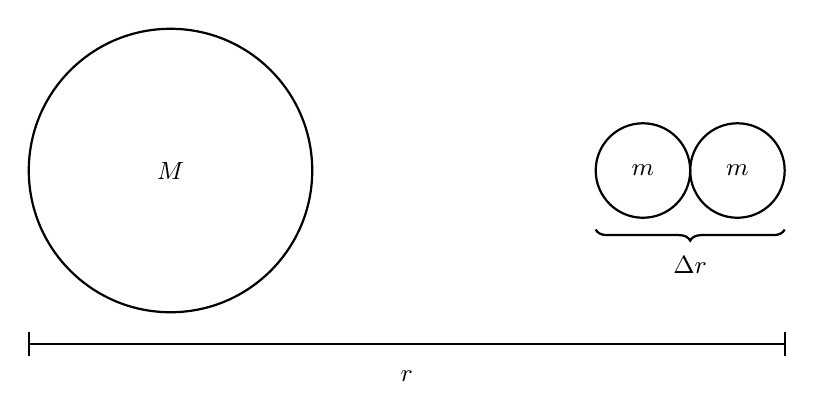
\begin{tikzpicture}[line width=0.8pt, every node/.style={font=\small}]
    %---- parameters you can tweak
    \def\R{1.8}   % radius of big mass M
    \def\r{0.60}  % radius of small masses m
    \def\gap{6.0} % center distance from M to the first small m
    \def\yd{-2.2} % vertical offset for the long dimension line
  
    %---- centers
    \coordinate (M)  at (0,0);
    \coordinate (m1) at (\gap,0);
    \coordinate (m2) at (\gap+2*\r,0); % touching m1
  
    %---- bodies
    \draw (M)  circle (\R);  \node at (M)  {$M$};
    \draw (m1) circle (\r);  \node at (m1) {$m$};
    \draw (m2) circle (\r);  \node at (m2) {$m$};
  
    %---- bracket for Δr across the two small masses
    \draw[decorate,decoration={brace,amplitude=4pt,mirror}]
      ($(m1)+(-\r,-1.25*\r)$) -- ($(m2)+(\r,-1.25*\r)$)
      node[midway,below=6pt] {$\Delta r$};
  
    %---- long dimension line r (with end ticks)
    \draw ($(M)+(-\R,\yd)$) -- ($(m2)+(\r,\yd)$);
    \draw ($(M)+(-\R,\yd)+(0,0.15)$) -- ++(0,-0.30);
    \draw ($(m2)+(\r,\yd)+(0,0.15)$) -- ++(0,-0.30);
   \node at ($($(M)+(-\R,\yd)$)!0.5!($(m2)+(\r,\yd)$)$) [below = 6pt] {$r$};
  
  \end{tikzpicture}
\end{center}


\subsection{Hill radius}
\begin{list}{-}{}
\item tidal forces of sun on earth-moon systems means that there is a maximum orbital distance for the moon, if it is to remain bound to the earth
\end{list}



















\pagebreak
\section{Glossary}

\textbf{\large Synodic period }

\begin{list}{-}{}
\item time elapsed between success conjunctions or oppositions
\item this is the period we observe from earth, which is moving
\end{list}
\noindent
\textbf{\large Sidereal Period} 
\begin{list}{-}{}
\item elapsed time of full orbit relative to the fixed stars (inertial ref frame)
\item This is the one we will want to put in keplers laws
\end{list}


\end{document}